\section{Artefact removal for EEG data}




\begin{figure}[!htbp]
\minipage{.5\textwidth}%
\centering
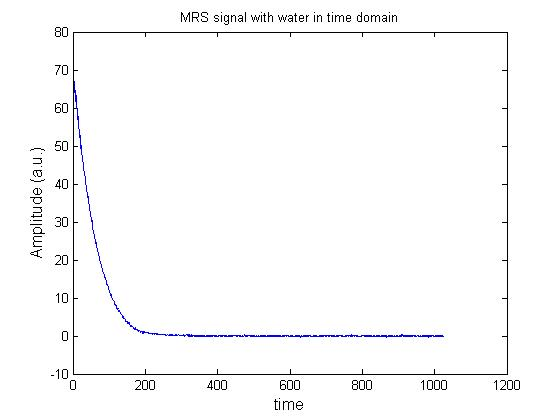
\includegraphics[width=.8\textwidth]{1.jpg}
\subcaption{EEG signal of the first set}
\endminipage\hfill
\minipage{.5\textwidth}%
\centering
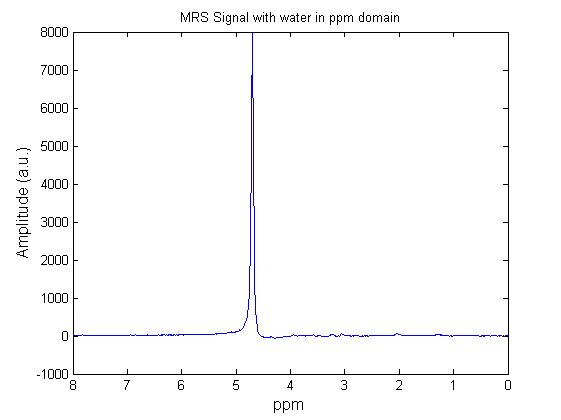
\includegraphics[width=.8\textwidth]{2.jpg}
\subcaption{EEG signal of the second set}
\endminipage\hfill
\caption{Orgininal EEG signals where in addition the most affected channels by the muscles artifacts are pointed out}
\end{figure}


\begin{figure}[!htbp]
\minipage{.3\textwidth}%
\centering
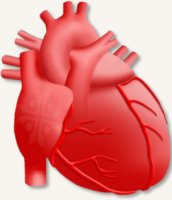
\includegraphics[width=1\textwidth]{3.jpg}
\subcaption{EEG reconstructed signals after CCA}
\endminipage\hfill
\minipage{.3\textwidth}%
\centering
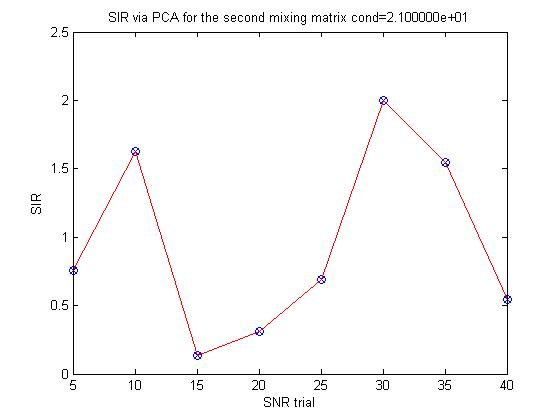
\includegraphics[width=1\textwidth]{4.jpg}
\subcaption{The CCA source channel}
\endminipage\hfill
\minipage{.3\textwidth}%
\centering
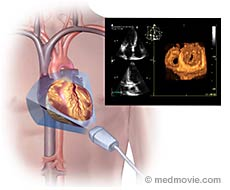
\includegraphics[width=1\textwidth]{5.jpg}
\subcaption{Correlation values for respective channel}
\endminipage\hfill
\caption{CCA outcome for the first data set}
\end{figure}

\begin{figure}[!htbp]
\minipage{.3\textwidth}%
\centering
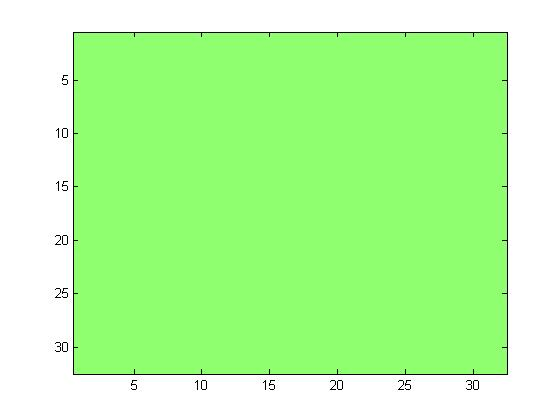
\includegraphics[width=1\textwidth]{6.jpg}
\subcaption{EEG reconstructed signals after CCA}
\endminipage\hfill
\minipage{.3\textwidth}%
\centering
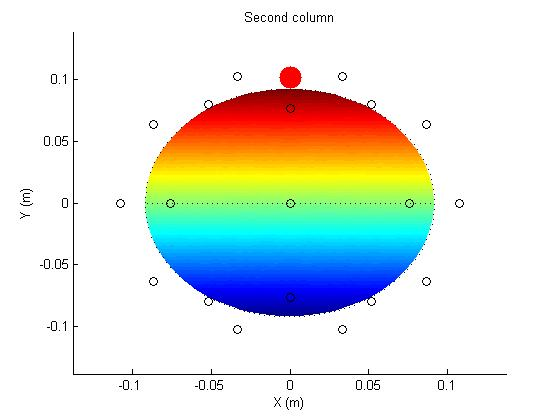
\includegraphics[width=1\textwidth]{7.jpg}
\subcaption{The CCA source channel}
\endminipage\hfill
\minipage{.3\textwidth}%
\centering
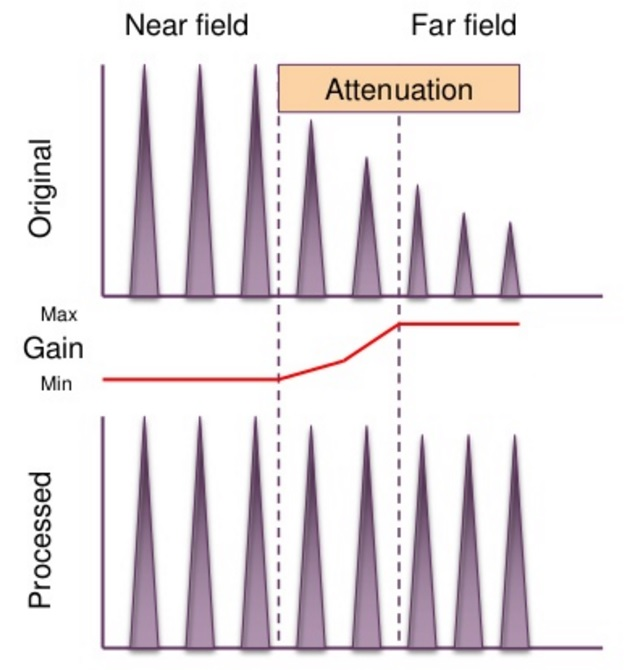
\includegraphics[width=1\textwidth]{8.jpg}
\subcaption{Correlation values for respective channel}
\endminipage\hfill
\caption{CCA outcome for the second data set}
\end{figure}

\begin{figure}[!htbp]
\minipage{.3\textwidth}%
\centering
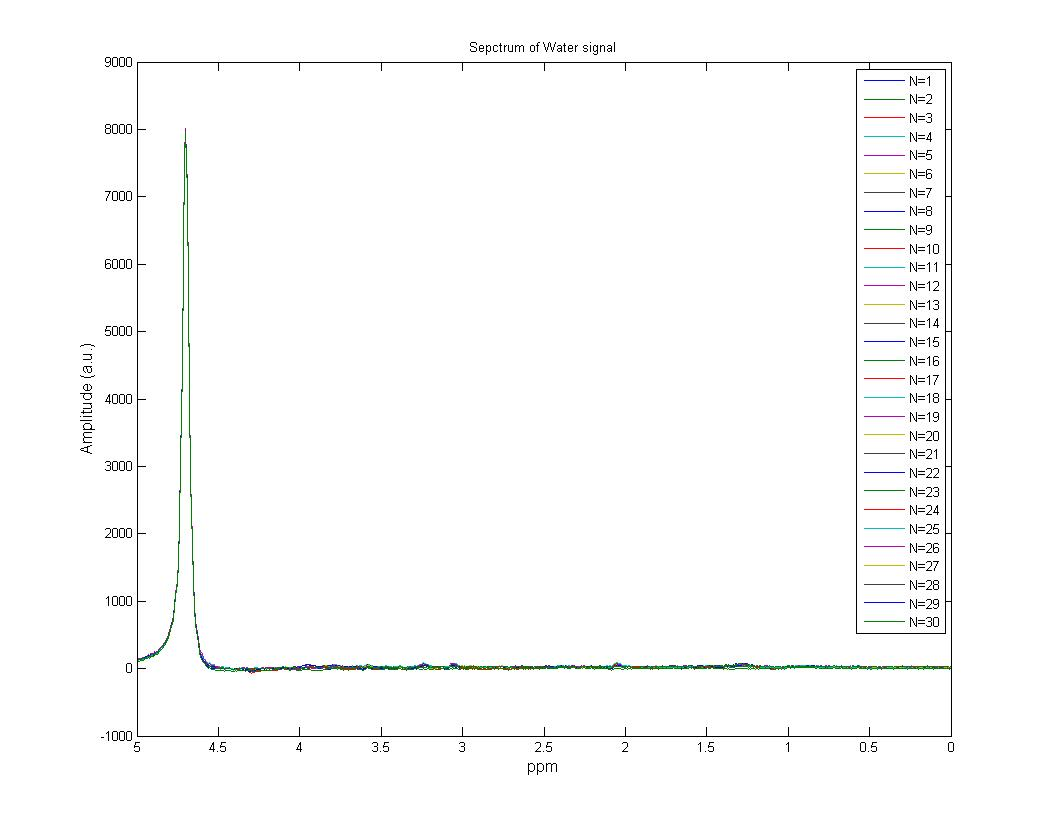
\includegraphics[width=1\textwidth]{9.jpg}\\
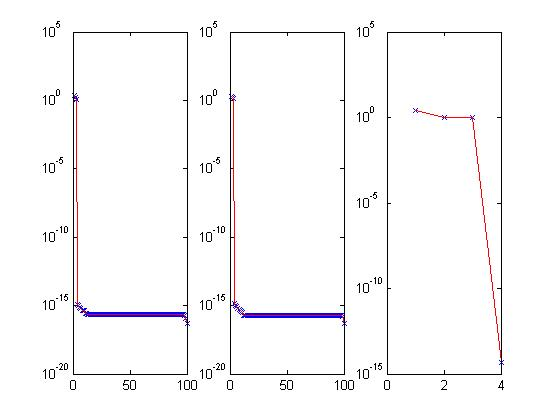
\includegraphics[width=1\textwidth]{10.jpg}
\endminipage\hfill
\minipage{.3\textwidth}%
\centering
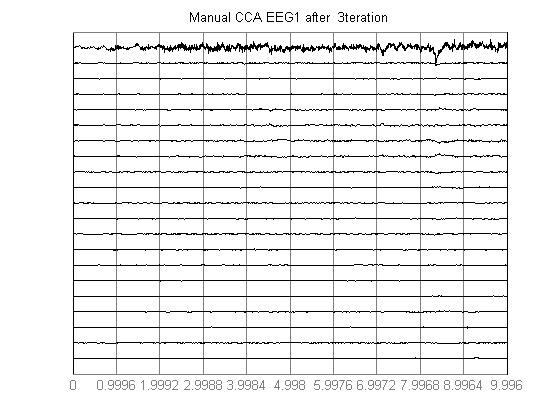
\includegraphics[width=1\textwidth]{11.jpg}\\
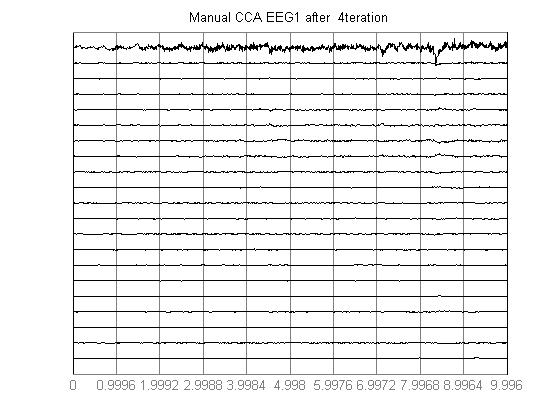
\includegraphics[width=1\textwidth]{12.jpg}
\endminipage\hfill
\minipage{.3\textwidth}%
\centering
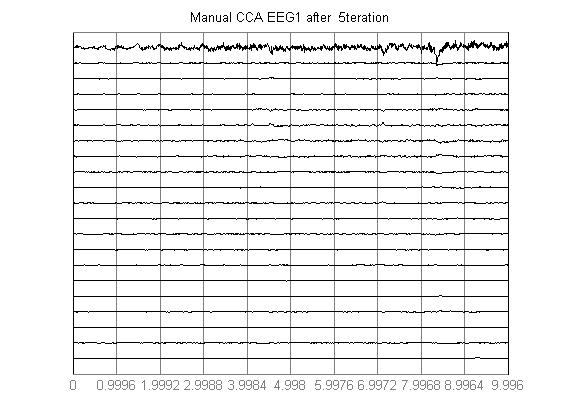
\includegraphics[width=1\textwidth]{13.jpg}\\
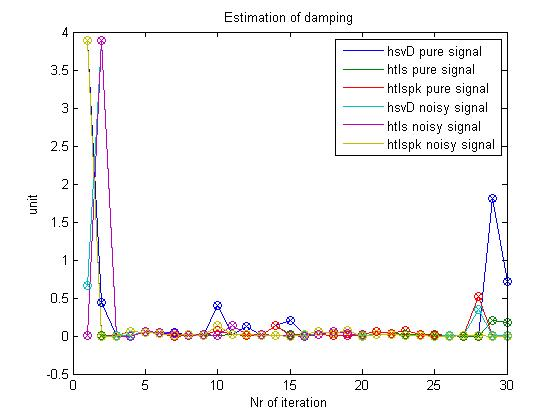
\includegraphics[width=1\textwidth]{14.jpg}
\endminipage\hfill
\caption{Manual CCA processing of the first EEG data set signal where the last plot outlines the noisy free EEG signal}\label{today4}
\end{figure}


\begin{figure}[!htbp]
\minipage{.3\textwidth}%
\centering
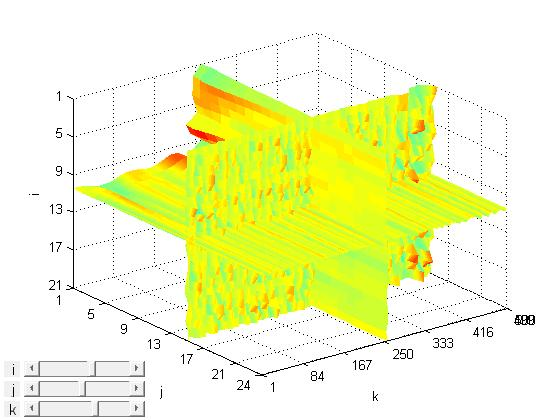
\includegraphics[width=1\textwidth]{16.jpg}\\
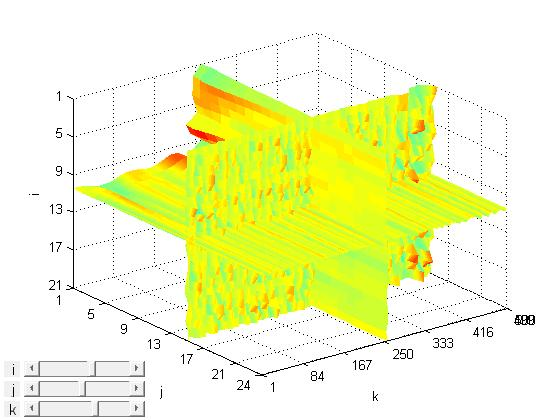
\includegraphics[width=1\textwidth]{16.jpg}\\
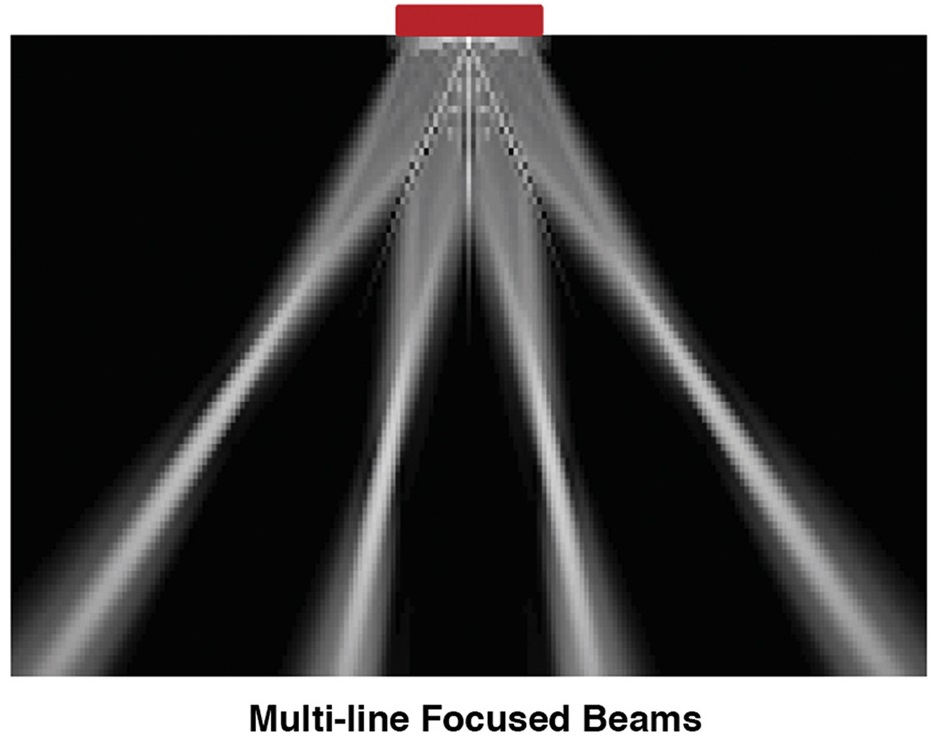
\includegraphics[width=1\textwidth]{17.jpg}\\
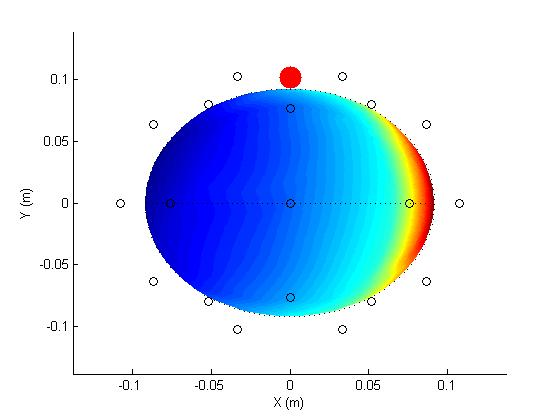
\includegraphics[width=1\textwidth]{18.jpg}
\endminipage\hfill
\minipage{.3\textwidth}%
\centering
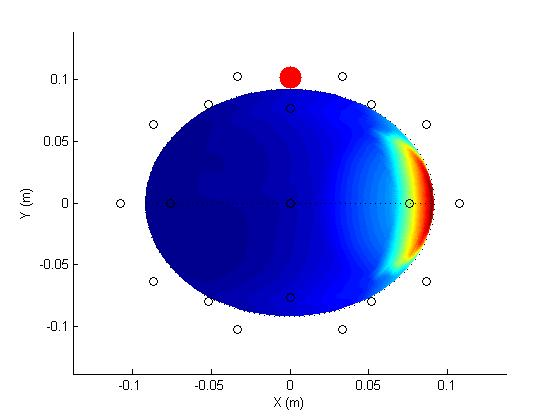
\includegraphics[width=1\textwidth]{19.jpg}\\
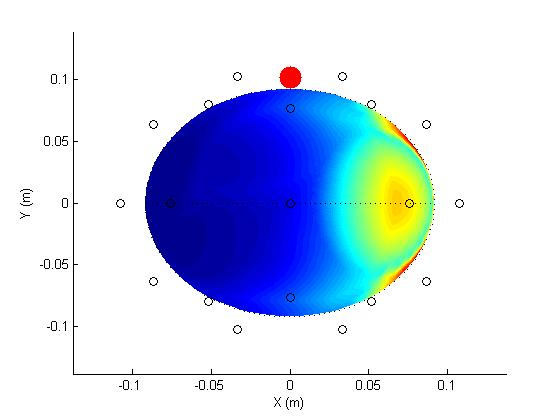
\includegraphics[width=1\textwidth]{20.jpg}\\
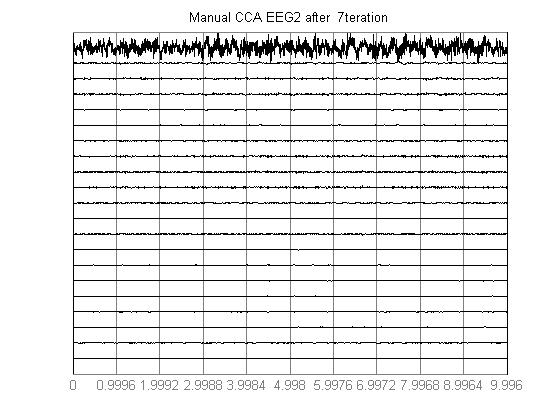
\includegraphics[width=1\textwidth]{21.jpg}\\
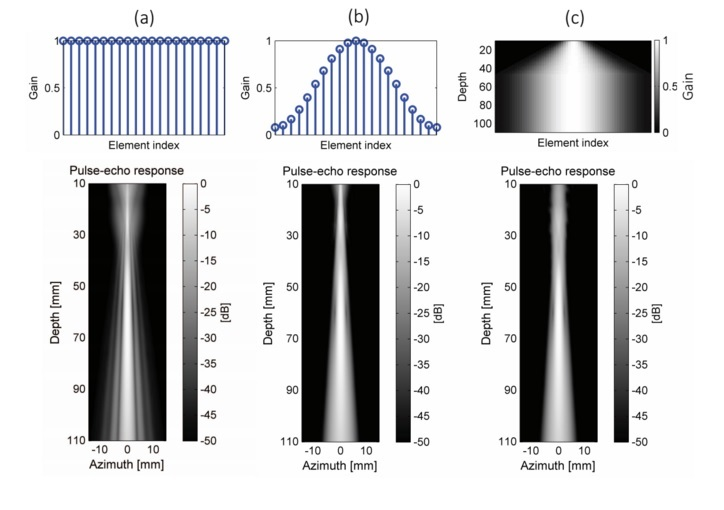
\includegraphics[width=1\textwidth]{22.jpg}
\endminipage\hfill
\minipage{.3\textwidth}%
\centering

\includegraphics[width=1\textwidth]{23.jpg}\\
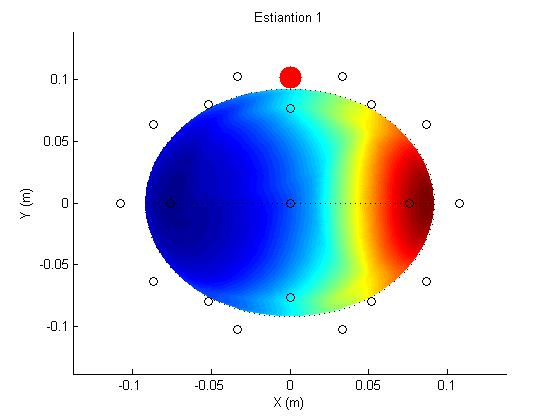
\includegraphics[width=1\textwidth]{24.jpg}\\
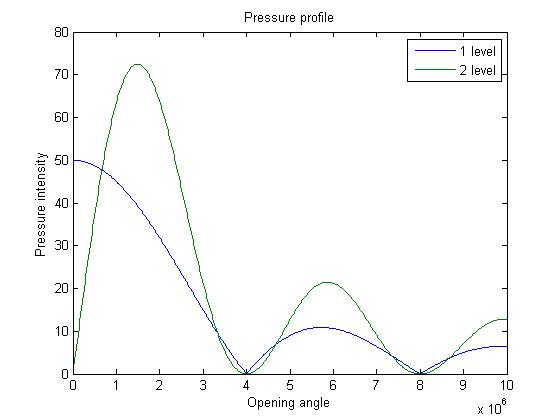
\includegraphics[width=1\textwidth]{25.jpg}\\
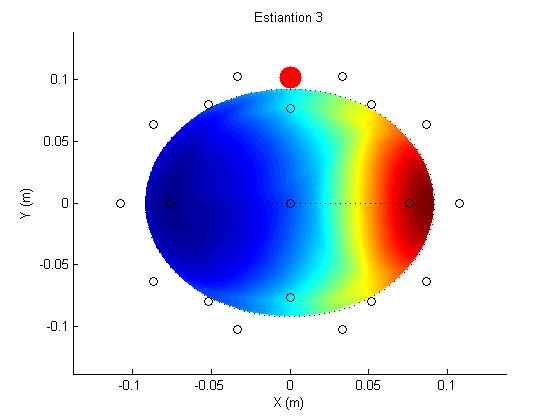
\includegraphics[width=1\textwidth]{26.jpg}
\endminipage\hfill
\caption{Manual CCA processing of the second EEG data set signal where the last plot outlines the noisy free EEG signal}\label{today3}
\end{figure}


\begin{figure}[!htbp]
\minipage{.5\textwidth}%
\centering
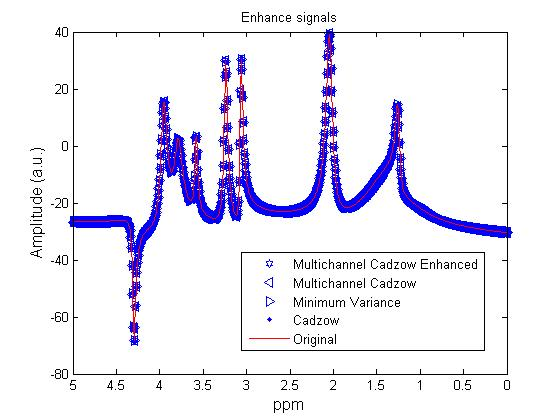
\includegraphics[width=1\textwidth]{27.jpg}
\subcaption{CCA results of the first data set}\label{toda1}
\endminipage\hfill
\minipage{.5\textwidth}%
\centering
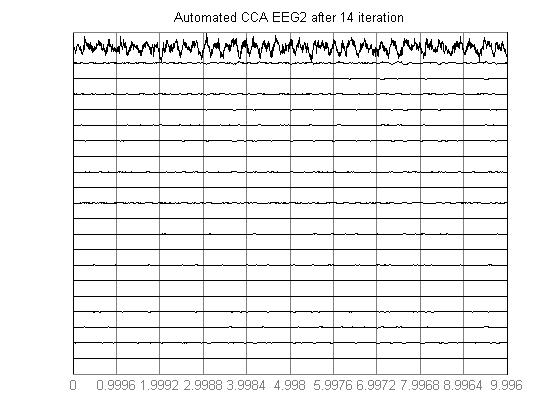
\includegraphics[width=1\textwidth]{28.jpg}
\subcaption{CCA results of the second data set}\label{toda2}
\endminipage\hfill
\caption{Automated processing of the CCA signals}
\end{figure}

CCA is very difficult to make it fully automated. Yet it is possible to make it semi automatic by erasing some of the channels where the correlation values is definitely without any influence into the signal. Moving into higher correlation values removing the channels manually increases the accuracy of the processing. Since this channels contain also information apart from the artifacts an accurate learning algorithm yet cannot decided precisely when to do this process. Nevertheless an automated method has been applied to remove the noisy signal by removing all those CCA channels where the correlation values is smaller than $0.7$. The results for this are outlined in the figure \ref{toda1} and \label{toda2} for the first and the second data set of the EEG signals. Whereas in the figure \ref{today3} and \ref{today4} are the manual results of the first and the second EEG data set. Furthermore the number of channels removed in the manual execution is much lower compare to the automatic case. This is the case because the visual classification is far better compare defining the the removed channel via the correlation coefficient.  

The two data set however contain different level of the artifact. The correlation coefficients for the first data set tends to sit into higher values compare to the second data set. Consequently the number of channels removed manually is much higher in the in the second data set. Even though the number of channels that are being removed are chosen manually, some  muscles artifact are hard to be removed via CCA. This is from the statistical backbone of the method which much of the information is "bonded" to the noisy quite "strongly" where statistical estimation cannot fully determine the relation between the two entities. The nosiy CCA channels are pointed out with anchor in both signals analysed. Artefacts usually arise randomly and at very high frequency compare to normal brain activities

\newpage
\subsection{Differences between CCA and ICA}


\begin{itemize}
\item CCA is an straight forward implementation, meaning that there is no need to iteratively solve or optimize any parameter. In the ICA case there is a need to diagonalize the the mixing matrix in order to make the channel data as much independent as possible \cite{15}. Although ICA is not a gradient based algorithm thus it is an fairly simple implementation when it comes in implementation but with a much higher time complexity compare to CCA. CCA employs either eigenvalues or singular values decomposition at a single iteration.  

\item In the ICA implementation there is no guarantee on the same output for identical data contrary to the CCA. This is mainly due to the fact that ICA outcome depends on the diagonalization process which is generally not predictable upon the accuracy require. In the CCA implementation both of the existing solution implementations\cite{16} the flow is independent of the type of the data set. Meaning that outcome arises at one iteration. The outcome of the ICA strictly depend on the data set values meaning that optimization process and the number of iteration has a certain variability. 

\item Even though both of the methods try to separate the sources the consideration is different in both cases. CCA tries to made the sources as less uncorrelated as possible whereas ICA tries to makes the sources as less independent as possible. Statistically speaking, independence is far stronger the uncorrelatedness meaning that independence implies the uncorrelatedness whereas the other way around does not stand. In other wards uncorrelatedness is just another weaker form for the independence\cite{15}. This two relations are equationed in equ.\ref{equati1} and equ.\ref{equati2}.

\item Differently from the CCA case, ICA assumes the input data set to be full non-Gaussian\cite{15}. Even though the nature events rarely contradict with the central limit theory, is some biomedical signal in particular non-Gaussianity is still no prevalent. CCA does not depend on this assumption, thereby it performs the separation at any type signals which are non correlated.

\item ICA could be seen from two different prospective. Commonly speaking the majority of the implementation tries to make them as much independent as possible. From the statistical point of view this is seen as diagonalizing the mixing matrix. In the information theory prospective this could be seen as well as the minimum mutual information between the sources\cite{15}. CCA does not offer this opportunity due to the weak Independence of the signal assumed in the uncorrelatedness.   

\item ICA in addition requires pre-processing  of the data, including here centering and whitening of the data\cite{15}. CCA does the separation straight from the raw data without the need of any pre-processing. Despite the pre-processing incorporated into the ICA, he still tends to be reluctant to the robustness due to the the assumption of neg-entropy and kurtosis estimation for the non Gaussianity \cite{17}. 

\item Auto-correlation is a well defined method thereby the correlation coefficient between the sources to be proceeded are defined very accurately in a very robust manner. The outcome is afterwards linearly processed with the aim of a separation of the sources. Whereas in the ICA the Independence is remains solid in multiple prospective. It could be ambiguous sometimes for application regarding the its implementation. 

\end{itemize}